% Created 2019-04-28 日 19:14
% Intended LaTeX compiler: pdflatex
\documentclass[11pt]{article}
\usepackage[utf8]{inputenc}
\usepackage[T1]{fontenc}
\usepackage{graphicx}
\usepackage{grffile}
\usepackage{longtable}
\usepackage{wrapfig}
\usepackage{rotating}
\usepackage[normalem]{ulem}
\usepackage{amsmath}
\usepackage{textcomp}
\usepackage{amssymb}
\usepackage{capt-of}
\usepackage{hyperref}
\usepackage{minted}
\usepackage{tikz,qtree}
\usepackage{forest,syntax}
% TIPS
% \substack{a\\b} for multiple lines text





% pdfplots will load xolor automatically without option
\usepackage[dvipsnames]{xcolor}

\usepackage{forest}
% two-line text in node by [two \\ lines]
% \begin{forest} qtree, [..] \end{forest}
\forestset{
  qtree/.style={
    baseline,
    for tree={
      parent anchor=south,
      child anchor=north,
      align=center,
      inner sep=1pt,
    }}}
%\usepackage{flexisym}
% load order of mathtools and mathabx, otherwise conflict overbrace

\usepackage{mathtools}
%\usepackage{fourier}
\usepackage{pgfplots}
\usepackage{amsthm}
\usepackage{amsmath}
%\usepackage{unicode-math}
%
\usepackage{commath}
%\usepackage{,  , }
\usepackage{amsfonts}
\usepackage{amssymb}
% importing symbols https://tex.stackexchange.com/questions/14386/importing-a-single-symbol-from-a-different-font
%mathabx change every symbol
% use instead stmaryrd
%\usepackage{mathabx}
\usepackage{stmaryrd}
\usepackage{empheq}
\usepackage{tikz}
\usepackage{tikz-cd}
%\usepackage[notextcomp]{stix}
\usetikzlibrary{arrows.meta}
\usepackage[most]{tcolorbox}
%\utilde
%\usepackage{../../latexpackage/undertilde/undertilde}
% left and right superscript and subscript
\usepackage{actuarialsymbol}
\usepackage{threeparttable}
\usepackage{scalerel,stackengine}
\usepackage{stackrel}
% \stackrel[a]{b}{c}
\usepackage{dsfont}
% text font
\usepackage{newpxtext}
%\usepackage{newpxmath}

%\newcounter{dummy} \numberwithin{dummy}{section}
\newtheorem{dummy}{dummy}[section]
\theoremstyle{definition}
\newtheorem{definition}[dummy]{Definition}
\newtheorem{corollary}[dummy]{Corollary}
\newtheorem{lemma}[dummy]{Lemma}
\newtheorem{proposition}[dummy]{Proposition}
\newtheorem{theorem}[dummy]{Theorem}
\theoremstyle{definition}
\newtheorem{example}[dummy]{Example}
\theoremstyle{remark}
\newtheorem*{remark}{Remark}


\newcommand\what[1]{\ThisStyle{%
    \setbox0=\hbox{$\SavedStyle#1$}%
    \stackengine{-1.0\ht0+.5pt}{$\SavedStyle#1$}{%
      \stretchto{\scaleto{\SavedStyle\mkern.15mu\char'136}{2.6\wd0}}{1.4\ht0}%
    }{O}{c}{F}{T}{S}%
  }
}

\newcommand\wtilde[1]{\ThisStyle{%
    \setbox0=\hbox{$\SavedStyle#1$}%
    \stackengine{-.1\LMpt}{$\SavedStyle#1$}{%
      \stretchto{\scaleto{\SavedStyle\mkern.2mu\AC}{.5150\wd0}}{.6\ht0}%
    }{O}{c}{F}{T}{S}%
  }
}

\newcommand\wbar[1]{\ThisStyle{%
    \setbox0=\hbox{$\SavedStyle#1$}%
    \stackengine{.5pt+\LMpt}{$\SavedStyle#1$}{%
      \rule{\wd0}{\dimexpr.3\LMpt+.3pt}%
    }{O}{c}{F}{T}{S}%
  }
}

\newcommand{\bl}[1] {\boldsymbol{#1}}
\newcommand{\Wt}[1] {\stackrel{\sim}{\smash{#1}\rule{0pt}{1.1ex}}}
\newcommand{\wt}[1] {\widetilde{#1}}
\newcommand{\tf}[1] {\textbf{#1}}


%For boxed texts in align, use Aboxed{}
%otherwise use boxed{}

\DeclareMathSymbol{\widehatsym}{\mathord}{largesymbols}{"62}
\newcommand\lowerwidehatsym{%
  \text{\smash{\raisebox{-1.3ex}{%
    $\widehatsym$}}}}
\newcommand\fixwidehat[1]{%
  \mathchoice
    {\accentset{\displaystyle\lowerwidehatsym}{#1}}
    {\accentset{\textstyle\lowerwidehatsym}{#1}}
    {\accentset{\scriptstyle\lowerwidehatsym}{#1}}
    {\accentset{\scriptscriptstyle\lowerwidehatsym}{#1}}
}

\usepackage{graphicx}
    
% text on arrow for xRightarrow
\makeatletter
%\newcommand{\xRightarrow}[2][]{\ext@arrow 0359\Rightarrowfill@{#1}{#2}}
\makeatother


\newcommand{\dom}[1]{%
\mathrm{dom}{(#1)}
}

% Roman numerals
\makeatletter
\newcommand*{\rom}[1]{\expandafter\@slowromancap\romannumeral #1@}
\makeatother

\def \fR {\mathfrak{R}}
\def \bx {\boldsymbol{x}}
\def \bz {\boldsymbol{z}}
\def \ba {\boldsymbol{a}}
\def \bh {\boldsymbol{h}}
\def \bo {\boldsymbol{o}}
\def \bU {\boldsymbol{U}}
\def \bc {\boldsymbol{c}}
\def \bV {\boldsymbol{V}}
\def \bI {\boldsymbol{I}}
\def \bK {\boldsymbol{K}}
\def \bt {\boldsymbol{t}}
\def \bb {\boldsymbol{b}}
\def \bA {\boldsymbol{A}}
\def \bX {\boldsymbol{X}}
\def \bu {\boldsymbol{u}}
\def \bS {\boldsymbol{S}}
\def \bZ {\boldsymbol{Z}}
\def \bz {\boldsymbol{z}}
\def \by {\boldsymbol{y}}
\def \bw {\boldsymbol{w}}
\def \bT {\boldsymbol{T}}
\def \bF {\boldsymbol{F}}
\def \bS {\boldsymbol{S}}
\def \bm {\boldsymbol{m}}
\def \bW {\boldsymbol{W}}
\def \bR {\boldsymbol{R}}
\def \bQ {\boldsymbol{Q}}
\def \bS {\boldsymbol{S}}
\def \bP {\boldsymbol{P}}
\def \bT {\boldsymbol{T}}
\def \bY {\boldsymbol{Y}}
\def \bH {\boldsymbol{H}}
\def \bB {\boldsymbol{B}}
\def \blambda {\boldsymbol{\lambda}}
\def \bPhi {\boldsymbol{\Phi}}
\def \btheta {\boldsymbol{\theta}}
\def \bTheta {\boldsymbol{\Theta}}
\def \bmu {\boldsymbol{\mu}}
\def \bphi {\boldsymbol{\phi}}
\def \bSigma {\boldsymbol{\Sigma}}
\def \lb {\left\{}
\def \rb {\right\}}
\def \la {\langle}
\def \ra {\rangle}
\def \caln {\mathcal{N}}
\def \dissum {\displaystyle\Sigma}
\def \dispro {\displaystyle\prod}
\def \E {\mathbb{E}}
\def \Q {\mathbb{Q}}
\def \N {\mathbb{N}}
\def \V {\mathbb{V}}
\def \R {\mathbb{R}}
\def \P {\mathbb{P}}
\def \A {\mathbb{A}}
\def \Z {\mathbb{Z}}
\def \I {\mathbb{I}}
\def \C {\mathbb{C}}
\def \cala {\mathcal{A}}
\def \calb {\mathcal{B}}
\def \calq {\mathcal{Q}}
\def \calp {\mathcal{P}}
\def \cals {\mathcal{S}}
\def \calg {\mathcal{G}}
\def \caln {\mathcal{N}}
\def \calr {\mathcal{R}}
\def \calm {\mathcal{M}}
\def \calc {\mathcal{C}}
\def \calf {\mathcal{F}}
\def \calk {\mathcal{K}}
\def \call {\mathcal{L}}
\def \calu {\mathcal{U}}
\def \bcup {\bigcup}


\def \uin {\underline{\in}}
\def \oin {\overline{\in}}
\def \uR {\underline{R}}
\def \oR {\overline{R}}
\def \uP {\underline{P}}
\def \oP {\overline{P}}

\def \Ra {\Rightarrow}

\def \e {\enspace}

\def \sgn {\operatorname{sgn}}
\def \gen {\operatorname{gen}}
\def \ker {\operatorname{ker}}
\def \im {\operatorname{im}}

\def \tril {\triangleleft}

% \varprod
\DeclareSymbolFont{largesymbolsA}{U}{txexa}{m}{n}
\DeclareMathSymbol{\varprod}{\mathop}{largesymbolsA}{16}

% \bigtimes
\DeclareFontFamily{U}{mathx}{\hyphenchar\font45}
\DeclareFontShape{U}{mathx}{m}{n}{
      <5> <6> <7> <8> <9> <10>
      <10.95> <12> <14.4> <17.28> <20.74> <24.88>
      mathx10
      }{}
\DeclareSymbolFont{mathx}{U}{mathx}{m}{n}
\DeclareMathSymbol{\bigtimes}{1}{mathx}{"91}
% \odiv
\DeclareFontFamily{U}{matha}{\hyphenchar\font45}
\DeclareFontShape{U}{matha}{m}{n}{
      <5> <6> <7> <8> <9> <10> gen * matha
      <10.95> matha10 <12> <14.4> <17.28> <20.74> <24.88> matha12
      }{}
\DeclareSymbolFont{matha}{U}{matha}{m}{n}
\DeclareMathSymbol{\odiv}         {2}{matha}{"63}


\newcommand\subsetsim{\mathrel{%
  \ooalign{\raise0.2ex\hbox{\scalebox{0.9}{$\subset$}}\cr\hidewidth\raise-0.85ex\hbox{\scalebox{0.9}{$\sim$}}\hidewidth\cr}}}
\newcommand\simsubset{\mathrel{%
  \ooalign{\raise-0.2ex\hbox{\scalebox{0.9}{$\subset$}}\cr\hidewidth\raise0.75ex\hbox{\scalebox{0.9}{$\sim$}}\hidewidth\cr}}}

\newcommand\simsubsetsim{\mathrel{%
  \ooalign{\raise0ex\hbox{\scalebox{0.8}{$\subset$}}\cr\hidewidth\raise1ex\hbox{\scalebox{0.75}{$\sim$}}\hidewidth\cr\raise-0.95ex\hbox{\scalebox{0.8}{$\sim$}}\cr\hidewidth}}}
\newcommand{\stcomp}[1]{{#1}^{\mathsf{c}}}


\graphicspath{{../../images/Compiler/}}
\author{wugouzi}
\date{\today}
\title{Compiler}
\hypersetup{
 pdfauthor={wugouzi},
 pdftitle={Compiler},
 pdfkeywords={},
 pdfsubject={},
 pdfcreator={Emacs 26.1 (Org mode 9.1.14)}, 
 pdflang={English}}
\begin{document}

\maketitle
\tableofcontents


\section{Chap1 introduction}
\label{sec:org2701f3e}
source code -> scanner -> [tokens] -> parser -> [syntax tree] -> semantic
analyzer -> [annotated tree] -> source code optimizer -> [intermediate code]
-> code generator -> [target code] -> target code optimizer -> [target code]

\section{chap2 scanning}
\label{sec:org1e9ba9b}
source code(\textbf{character stream}) -> \textbf{token stream}. Use regular expression.
a ε R|S RS R* R+=R(R*) R?=(R|ε) [abce]=(a|b|c|e) [a-z] [\(^{\text{az}}\)]=anything but
one of the listed chars

comment "\emph{*"([\(^{\text{*}}\)/]|[\(^{\text{*}}\)]"}"|"\textbf{"[\^{}/])}"*/"

finite automata

Thompson's construction


Minimizing the number of states in a DFA
\begin{enumerate}
\item it begins with the most optimistic assumptions possible: it create two sets
\begin{itemize}
\item one consisting of all the accepting states
\item the other consisting of all the nonaccepting states
\end{itemize}
\item given this partition of the states of the original DFA, consider the
transitions on \textbf{each character} a of the alphabet
\begin{itemize}
\item if all accepting states have transitions on a to accepting states,
defines an a-transition from the new accepting state to itself
\item if all accepting states have transitions on a to nonaccepting states \ldots{}
\end{itemize}
\item given this partition of the states of the original DFA, consider the
transitions on each character a of the alphabet
\begin{itemize}
\item if there are two accepting states s and t that have transitions on a that
land in different sets, no a-transition can be defined for this grouping
of the states. a distinguish the states s and t
\item if there are two accpeting states s and t s.t. s has an a-transition to
another accepting state, while t has no a-transition at all. a
distinguish s and t
\end{itemize}
\end{enumerate}

\section{Chap3 context-free grammars and parsing}
\label{sec:org789c8a4}
\subsection{context-free grammars}
\label{sec:orge72ae2c}
A context-free grammar involves recursion rules. 4-tuple \((V,\Sigma,S,\to)\).
V nonterminal. Σ terminal. S start symbol. \(\to\subset
   V\times(V\cup\Sigma)*\)

\textbf{Left recursive}: the nonterminal A appears as the first symbol on the
right-hand side of the rule defining A

\textbf{Right recusive}:

\textbf{ε-production}: empty->ε
A grammar that generates a language containing the empty string must have at
least one \textbf{ε-production}
\subsection{Parse tree and abstract syntax trees}
\label{sec:org7d4cd5c}
\subsubsection{parse tree}
\label{sec:org5263ef9}
A \textbf{parse tree} corresponding to a derivation is a labeled tree
\begin{itemize}
\item the interior nodes are labeled by \textbf{nonterminals}
\item the leaf is \textbf{terminals}
\end{itemize}

\textbf{left-most derivation}
\subsubsection{abstract symtax tree}
\label{sec:org4b24caf}
\begin{forest}
[+ [3] [4] ]
\end{forest}
\subsection{Ambiguity}
\label{sec:org6116cd5}
\subsubsection{ambiguity grammars}
\label{sec:orgdf8b044}
\textbf{ambiguous grammar}: a grammar that generates a string with two distinct parse
trees

Two basic methods:
\begin{enumerate}
\item A rule: that specifies in each ambiguous case which of the parse trees is
the correct one. \textbf{disambbiguating rule}
\begin{itemize}
\item associativity
\end{itemize}
\item change the grammar
\end{enumerate}
\subsubsection{precedence and associativity}
\label{sec:org1272b82}
A \emph{left recursive} rule makes its operators associate on the left
\subsubsection{the dangling else problem}
\label{sec:org933b428}
\begin{grammar}
<statement> ::= <if-stmt>
\alt `other'

<if-stmt> ::= `if' `(' <exp> `)' <statement>
\alt `if' `(' <exp> `)' <statement> `else' <statement>
\end{grammar}

disambiguating rule is \textbf{most closely nested rule}.
grammar is
\begin{grammar}
<statement> -> <matched-stmt>
\alt <unmatched-stmt>

<matched-stmt> -> `if' `(' <exp> `)' <matched-stmt> `else' <matched-stmt>
\alt `other'

<unmatched-stmt> -> `if' `(' <exp> `)' <statement>
\alt `if' `(' <exp> `)' <matched-stmt> `else' <unmatched-stmt>

<exp> -> `0'
\alt `1'
\end{grammar}
\subsubsection{inessential ambiguity}
\label{sec:orgd93290c}
sometimes a grammar may be ambiguous and yet always produce unique \emph{abstract}
\emph{syntax tree}.

\textbf{inessential ambiguity}: the associated semantics don't depend on what
 disambiguating rule is used
\subsubsection{extended notations: EBNF and syntax diagrams}
\label{sec:org00eb3e2}
\(A\to A\;\alpha\mid\beta\Longrightarrow A\to\beta\;\{\alpha\}\).
\(A\to\alpha\; A\mid\beta\Longrightarrow A\to\{\alpha\}\;\beta\)
\subsection{Formal properties of context-free language}
\label{sec:orgb147042}
A context-free grammar consists of the following
\begin{enumerate}
\item T terminals
\item N nonterminals
\item P grammar rules
\item S start symbol
\end{enumerate}

\textbf{sentential form} a string a in \((T\cup N)*\)

A grammar G is \textbf{ambiguous} if there exists a string \(w\in L(G)\) s.t. w has two
distinct parse trees

\section{Chap4 top-down parsing}
\label{sec:org1919f80}
\subsection{Top-down parsing by recursive-descent}
\label{sec:org032d95c}
not easy and use EBNF
\begin{grammar}
<if-stmt> ::= `if' `(' <exp> `)' <statement>
\alt `if' `(' <exp> `)' <statement> `else' <statement>
\end{grammar} to if-stmt -> if (exp) statement [else statement]
\subsection{LL(1) parsing}
\label{sec:org8623038}
use an explicit stack rather than recursive calls.
\begin{grammar}
<S> ::= <E> `+' <S>
\alt <E>

<E> ::= `num'
\alt `(' <S> `)'
\end{grammar}.
\begin{center}
\begin{tabular}{lrlr}
partly-derived string & lookahead & parsed part & unparsed part\\
\hline
S & ( &  & (1+2+(3+4))+5\\
E+S & ( &  & (1+2+(3+4))+5\\
(S)+S & 1 & ( & 1+2+(3+4))+5\\
(E+S)+S & 1 & ( & 1+2+(3+4))+5\\
(1+S)+S & 2 & (1+ & 2+(3+4))+5\\
(1+E+S)+S & 2 & (1+ & 2+(3+4))+5\\
(1+2+S)+S & ( & (1+2+( & (3+4))+5\\
\end{tabular}
\end{center}

For \(S\to(S)\; S\mid\epsilon\)
\begin{center}
\begin{tabular}{rlll}
step & parsing & input & action\\
\hline
1 & \$S & ()\$ & S->(S)S\\
2 & \$S)S( & ()\$ & match\\
3 & \$S)S & )\$ & S->e\\
4 & \$S) & )\$ & match\\
5 & \$S & \$ & S->e\\
6 & \$ & \$ & match\\
\end{tabular}
\end{center}

Two actions:
\begin{enumerate}
\item generate
\item match: match a token on top of the stack with the next input token
\end{enumerate}

This corresponds to the leftmost derivation. \textbf{characteristic of top-down
parsing}
\subsubsection{LL(1) parsing table}
\label{sec:org5719107}
parsing table
\begin{center}
\begin{tabular}{llll}
M[N,T] & ( & ) & \$\\
\hline
S & S->(S)S & S->e & S->e\\
\end{tabular}
\end{center}

M is the set of non-terminals.
T is the set of terminals or tokens including \$

Table-constructing rule:
\begin{enumerate}
\item if \(A\to\alpha\) is a production choice and there is a derivation
\(\alpha\Rightarrow*a\beta\) where a is a token then add \(A\to\alpha\) to
M[A,a]
\item if \(A\to\alpha\) and
\(\alpha\Rightarrow*\epsilon,S\textdollar\textsterling\Rightarrow^*\beta
      Aa\gamma\), where S is the start symbol and a is a token(or \$), then add
\(A\to\alpha\) to M[A,a]
\end{enumerate}

A grammar is LL(1) if LL(1) parsing table has at most one production in each entry
\subsubsection{left recursion removal and left factoring}
\label{sec:org0a03681}
\textbf{left recursion removal}
\begin{itemize}
\item \textbf{immediate left recursion}: \(exp\to exp\;+\;term|exp\;-\;term|term\)
\item \textbf{indirect left recursion}: \(A\to Bb\) and \(B\to Aa\)
\end{itemize}


\begin{enumerate}
\item Simple immediate left recursion.
\(A\to A\alpha|\beta\) to \(A\to\beta\;A'\) and \(A'\to\alpha\;A'|\epsilon\)
\item general immediate left recursion.
\(A\to A\alpha_1|\dots|A\alpha_n|\beta_1|\dots|\beta_m\) to
\(A\to\beta_1A'|\dots|\beta_mA'\) and
\(A'\to\alpha_1A'|\dots|\alpha_nA'|\epsilon\)
\item general left recursion. grammars with no \$\(\epsilon\)\$-productions and no cycles
\end{enumerate}


doesn't change language, but changes the grammar and parse tree

\textbf{left factoring}.
\(A\to\alpha\beta|\alpha\gamma\) to \(A\to\alpha A'\) and \(A'\to\beta\mid\gamma\)
\subsubsection{Syntax tree construction in LL(1) parsing}
\label{sec:org4599d70}
\subsection{First and follow sets}
\label{sec:orgd8dee89}
X a grammar symbol(a terminal or non-terminal) or \(\epsilon\). Then First(X)
is 
\begin{enumerate}
\item if X is a terminal or \(\epsilon\), then First(X)=\{X\}
\item if X is a non-terminal, for each \(X\to X_1X_2\dots X_n\), First(X) contains
First(X1) - \{e\}
\end{enumerate}

A non-terminal A is \textbf{nullable} iff there exists \(A\Rightarrow^*\epsilon\) iff
First(A) contains \(\epsilon\)

Follow(A) is 
\begin{enumerate}
\item if A is start symbol, \$ is in Follow(A)
\item if \(B\to\alpha A\gamma\), then
\(\text{First}(\gamma)-\{\epsilon\}\subseteq\text{Follow}(A)\)
\item if \(B\to\alpha A\gamma, \epsilon\in\text{First}(\gamma)\), then Follow(A)
contains Follow(B)
\end{enumerate}
\subsection{Error recovery in top-down parsers}
\label{sec:org97772f6}
\section{Chap5 Bottom-up parsing}
\label{sec:org8607675}
\subsection{Overview of bottom-up parsing}
\label{sec:org1920ee8}
\begin{itemize}
\item A bottom-up parser uses an \textbf{explicit stack} to perform a parse
\item The parsing stack will contain both tokens and nonterminals
\begin{center}
\begin{tabular}{ll}
\$ & inputstring \$\\
\hline
\ldots{} & \ldots{}\\
\$StartSymbol & \$accept\\
\end{tabular}
\end{center}
\item \textbf{right-most} derivation -- backward
start with the tokens; end with the start symbol
\begin{center}
\begin{tabular}{l}
(1+2+(3+4))+5\\
(E+2+(3+4))+5\\
(S+2+(3+4))+5\\
(S+E+(3+4))+5\\
(S+(3+4))+5\\
(S+(E+4))+5\\
(S+(S+4))+5\\
(S+(S+E))+5\\
(S+(S))+5\\
(S+E)+5\\
(S)+5\\
E+5\\
S+5\\
S+E\\
S\\
\end{tabular}
\end{center}
\item \textbf{parsing actions}: a sequence of \textbf{shift} and \textbf{reduce} operations
\textbf{parser state}: a stack of terminals and non-terminals
\textbf{current derivation step} = always stack + input
\begin{center}
\begin{tabular}{llr}
derivation & step stack & unconsumed input\\
\hline
(1+2+(3+4))+5 &  & (1+2+(3+4))+5\\
 & ( & 1+2+(3+4))+5\\
(E+2+(3+4))+5 & (E & +2+(3+4))+5\\
(S+2+(3+4))+5 & (S & +2+(3+4))+5\\
 & (S+ & 2+(3+4))+5\\
 & (S+2 & +(3+4))+5\\
(S+E+(3+4))+5 & (S+E & +(3+4))+5\\
\end{tabular}
\end{center}
\item 1. \textbf{shift}: shift a terminal from the front of the input to the top of the
stack 
\begin{enumerate}
\item \textbf{reduce}: reduce a string α at the top of the stack to a nonterminal A,
given the BNF choice A ⟶ α
\end{enumerate}

A bottom-up parser: \textbf{shift-reduce parser}
\item One further feature of bottom-up parsers: grammars are always augmented
with a \textbf{new start symbol}. if S is the start symbol, a new start symbol S' is
added to the grammar :  S' →S

\item example

S'->S

S ->(S)S|e

S'=>S=>(S)S=>(S)=>()
\begin{center}
\begin{tabular}{rlrl}
 & Parsing stack & Input & Action\\
\hline
1 & \$ & ( ) \$ & Shift\\
2 & \$ ( & ) \$ & Reduce  S -> ε\\
3 & \$ (S & ) \$ & Shift\\
4 & \$ (S ) & \$ & Reduce  S -> ε\\
5 & \$ (S ) S & \$ & Reduce S --> (S) S\\
6 & \$S & \$ & Reduce S'--> S\\
7 & \$S' & \$ & Accept\\
\end{tabular}
\end{center}

\item example

E'->E

E->E+n|n

E'=>E=>E+n=>n+n
\begin{center}
\begin{tabular}{rlrl}
 & Parsing stack & Input & Action\\
1 & \$ & n+n\$ & Shift\\
2 & \$n & +n\$ & Reduce  E->n\\
3 & \$E & +n\$ & Shift\\
4 & \$E+ & n\$ & Shift\\
5 & \$E+n & \$ & Reduce E->E+n\\
6 & \$E & \$ & Reduce E'->E\\
7 & \$E' & \$ & Accept\\
\end{tabular}
\end{center}
\item[{Right sentential form}] \begin{itemize}
\item A \textbf{sentential} form is any string derivable from the start symbol. Note
that this includes the forms with non-terminals at intermediate steps as
well.
\item A \textbf{right-sentential form} is a sentential form that occurs in a step of
rightmost derivation (RMD). 
Each of the intermediate strings of terminals and nonterminals in such
a derivation is called a right sentential form
Each such sentential form is split between the parsing stack and the input
during a shift-reduce parse
\item A \textbf{sentence} is a sentential form consisting only of terminals
\end{itemize}

E,E+,E+n are \textbf{viable prefixes} of the right sentential form E+n.
The sequence of symbols on the parsing stack is called \textbf{viable prefix} of the
right sentential form
\item \textbf{handle}
This string, together with the \textbf{position} in the right sentential form where it
occurs, and the production used to reduced it, is called the \textbf{handle} of the right
sentential form

\uline{determining the next handle in a parse is the main task of a shift-reduce parser}
\end{itemize}
\subsection{Finite automata of LR(0) items and LR(0) parsing}
\label{sec:orga4c4207}
\begin{itemize}
\item An \textbf{LR(0) item} of a context-free grammar: a production choice with a
distinguished position in its right-hand side
\item If \textbf{A -> α}, \textbf{βγ = α}, then \textbf{A -> β · γ} is an LR(0) item
\item Example
\begin{center}
\begin{tabular}{l}
S' -> S\\
S -> (S)S $\backslash$ e\\
S' -> ·S\\
S' -> S·\\
S -> ·(S)S\\
S -> (·S)S\\
S -> (S·)S\\
S -> (S)·S\\
S -> (S)S·\\
S -> ·\\
\end{tabular}
\end{center}
\end{itemize}
\subsubsection{Finite automata of items}
\label{sec:orge2d13f7}
\begin{itemize}
\item The LR(0) items: as the state of a finite automata
\item construct the DFA of sets of LR(0) using the subset construction from NFA
\item If X is a token or a nonterminal

\begin{tikzpicture}
[place/.style={circle,minimum size=5mm}]
\node (x1) at (0,0) [place] {$A\to\alpha\cdot X\eta$};
\node (x2) at (5,0) [place] {$A\to\alpha X\cdot\eta$};
\draw [->] (x1) to node [above] {X} (x2);
\end{tikzpicture}
\item If X is a token, then this transition corresponds to a shift of X from the
input to the top of the stack during a parse
\item if X is a nonterminal,
X will never appear as an input symbol

\begin{tikzpicture}
\node (x1) at (0,0) [circle] {$A\to\alpha\cdot X\eta$};
\node (x2) at (5,0) [circle] {$X\to\cdot\beta$};
\draw [->] (x1) to node [above] {$\epsilon$} (x2);
\end{tikzpicture}
\item The \textbf{start state} of the NFA ↔ the \textbf{initial state} of the parser: the stack is
empty
\item the solution is to augment the grammar by a single production S' -> S
\item \textbf{S'->·S} the \textbf{start state} of the NFA
\end{itemize}
\subsubsection{The LR(0) parsing algorithm}
\label{sec:orgfb08967}
\begin{itemize}
\item the parsing stack to store: \textbf{symbols} and \textbf{state numbers}
\item pushing the new \textbf{state number} onto the parsing stack after each push of \textbf{a
symbol}
\item Let s be the current state. Then actions are
\begin{enumerate}
\item if state s contains any item of the form \textbf{A -> α·Xβ} (X is a terminal).
Then the action is to shift the current input token onto the stack
\item If state s contains any \textbf{complete item} (an item of the form \textbf{A->γ·}),
then the action is to reduce by the rule \textbf{A->γ·}
\begin{itemize}
\item A \textbf{reduction} by the rule \textbf{S'->S} where S' is the start state
\item \textbf{acceptance} if the input is empty
\item \textbf{Error} if the input is not empty
\end{itemize}
\end{enumerate}
\item A grammar is \textbf{LR(0)} grammar if the above rules are unambiguous
\item A grammar is \textbf{LR(0)} iff
\begin{itemize}
\item Each state is a shift state
\item A reduce state containing a single complete item
\end{itemize}
\item table
\begin{center}
\begin{tabular}{rllrrlr}
state & action & rule & input & input & input & goto\\
\hline
 &  &  & ( & a & ) & A\\
0 & shift &  & 3 & 2 &  & 1\\
1 & reduce & A'->A &  &  &  & \\
2 & reduce & A->(A) &  &  &  & \\
3 & shift &  & 3 & 2 &  & 4\\
4 & shift &  &  &  & 5 & \\
5 & reduce & A->a &  &  &  & \\
\end{tabular}
\end{center}
\end{itemize}
\subsection{SLR(1) Parsing (simple LR(1))}
\label{sec:org33e2e22}
\begin{itemize}
\item \textbf{definition}
\begin{enumerate}
\item if state s contains any item of form \(A\to\alpha\cdot X\beta\), then the
action is to shift the current input token onto the stack, and the new
state to be pushed on the stack is the state containing the item
\(A\to\alpha\cdot X\beta\)
\item if state s contains the complete item \(A\to\gamma\cdot\), and \uline{the next token in}
\uline{the input string is in Follow(A)}, then the action is to reduce by the
rule \(A\to\gamma\)
\begin{itemize}
\item A reduction by the rule \textbf{S'->S} where S' is the start state, this will
happen only if the next input token is \$
\item remove the string γ and all of its corresponding states from the parsing
stack
\item back up in the DFA to the state from which the construction of γ begin
\item this state must contain an item of the form \(B\to\alpha\cdot A\beta\).
Push A to the stack, and push the state containing the item
\(B\to\alpha\cdot A\beta\)
\end{itemize}
\item if the next input token is s.t. neither of the above two cases applies,
an error is declared
\end{enumerate}
\item A grammar is \textbf{SLR(1)} iff for any state s
\begin{enumerate}
\item for any item \(A\to\alpha\cdot X\beta\) in s with X a terminal, there is no \uline{complete}
\uline{item} \(B\to\gamma\cdot\) in s with X ∈ Follow(B)
\item For any two complete item \(A\to\alpha\cdot\) and \(B\to\beta\cdot\) in s,
\(\text{Follow}(A)\cap\text{Follow(B)}=\emptyset\)
\end{enumerate}
\item right recursion can cause stack overflow
\end{itemize}
\subsubsection{disambiguating rules for parsing conflicts}
\label{sec:org15c60a2}
\begin{itemize}
\item two kinds of parsing conflicts in SLR(1) parsing
\textbf{shift-reduce} conflicts
\textbf{reduce-reduce} conflicts
\item in the case of shift-reduce conflicts, there is a natural
\textbf{disambiguaiting rule}: \uline{always prefer shift over the reduce}
\item 
\end{itemize}
\subsubsection{limits of SLR(1) parsing power}
\label{sec:org4c85ed5}
\subsection{General LR(1) and LALR(1) parsing}
\label{sec:orga96c539}

\begin{itemize}
\item the difficulty with the SLR(1) method:
applies lookaheads after the construction of the DFA of LR(0) items
\item An \textbf{LR(1)} item is a pair consisting of an \textbf{LR(0)} item and a \textbf{lookahead} token
\item \textbf{LR(1)} item as
\textbf{[A->α·β, a]}
A->α·β is LR(0) item, a is a token
\item \textbf{definition of LR(1) transitions} main difference of LR(0) and LR(1)
\textbf{[A->α·Xγ, a]}, X is any symbol, there is a transition on X to
\textbf{[A->αX·γ,a]}
\textbf{[A->α·Bγ,a]}, B nonterminal, there are ε-transitions to items \textbf{[B->·β,b]}
for every \textbf{B->β} and for every token b in \textbf{First(γa)}
\end{itemize}
\subsubsection{Finite automata of LR(1) items}
\label{sec:org08db46b}
\begin{itemize}
\item \textbf{start} state
S'->S
\item start item

\textbf{[S'->·S, \$]}
\end{itemize}
\subsubsection{The LR(1) parsing algorithm}
\label{sec:org572ae5c}
\begin{itemize}
\item the general LR(1) parsing algorithm
Let s be the current state.

\begin{enumerate}
\item s:[A->α·Xβ,a], X terminal, X is the next token in the input string \textbf{shift}
\item s: [A->α·,a], the next token in the input string is a \textbf{reduce}
\item otherwise error
\end{enumerate}
\item A grammar is \textbf{LR(1)} iff for any state s
\begin{enumerate}
\item for any item \textbf{[A->α·β,a]} in s with X a terminal, there is no item in s
of the form \textbf{[B->γ·,X]} (otherwise there is a \uline{shift-reduce} conflict
\item there are no two item in s of the form \textbf{[A->α·,a]} and \textbf{[B->β·,a]}
\end{enumerate}
\end{itemize}
\subsection{LALR(1) parsing}
\label{sec:org8bb033e}
\begin{itemize}
\item the size of the DFA of sets of LR(1) items is too large
\item first principle of LAIR(1) parsing
the core of a state of DFA of LR(1) is a state of the DFA of LR(0) items
\item second principle of LAIR(1) parsing
s₁,s₂ of DFA of LR(1) that have the same core, suppose there is a transition
on the symbol X from s₁ to a state t₁, then there is also a transition on X
from state s₂ to a state t₂, and the states t₁ and t₂ have the same core
\item if a grammar is LR(1) then the LALR(1) parsing table cannot have any
shift-reduce conflicts, there may be reduce-reduce conflicts
\item if a grammar is SLR(1), then it's LALR(1)
\item compute the DFA of LALR(1) items directly from the DFA of LR(0) items through
a process of \textbf{propagating lookaheads}
\end{itemize}
\subsection{Error recovery in Bottom-up parsers}
\label{sec:org6e973df}
A bottom-up parser will detect an error when a blank entry is detected
\section{chap6 semantics analysis}
\label{sec:orgfc3d8ad}
\subsection{Attributes and attribute grammars}
\label{sec:org3c0e916}
\textbf{attribute}: any property of a programming language constructs. May be fixed prior to
the compilation process or be only determinable during program execution

\textbf{binding} of the attribute: the process of computing an attribute and associating its
computed value with the language construct in question

\textbf{binding time}: the time during the compilation/execution process when the binding of
an attribute occurs

\textbf{static attributes/dynamic attributes}: based on the difference of the binding time

\textbf{type checker}: an analyzer.
computes the data type attribute of all language entities for which
data types are defined. And verifies that these types conform to the type rules of
the language

\textbf{type checking}: set of rules that ensure the type consistency of different constructs
in the program. e.g. operands types and so on
\subsubsection{attribute grammars}
\label{sec:org8cd4648}
\begin{itemize}
\item \(X.a\): the value of a associated to X

\(X\) is a grammar symbol and \(a\) is an attribute associated to \(X\)
\item \textbf{syntax-directed semantics}: attributes are associated directly with the grammar
symbols of the language
\item given attributes \(a_1, a_2,...,a_k\) for each grammar rule 
\(X_0\to X_1\dots X_n\), the values of
the attributes \(X_i.a_j\) of each grammar symbol \(X_i\) are related to the values of the
attributes of the other symbols in the rule
\item an \textbf{attribute grammar}

\(X_i.a_j=f_{ij}(X_0.a_1,\dots,X_0.a_k,\dots,X_n.a_1,\dots,X_n.a_k)\)
\item example

For 
\begin{grammar}
<number> ::= <number> <digit> \alt <digit>

<digit> ::= `[0123456789]'
\end{grammar}
\begin{center}
\begin{tabular}{ll}
grammar rule & semantic rules\\
\hline
\(number1 \to number2 \; digit\) & \(number1.val=number2.val\times 10+digit.val\)\\
\(number\to digit\) & \(number.val=digit.val\)\\
\(digit\to 0\) & \(digit.val=0\)\\
\end{tabular}
\end{center}
\end{itemize}


\begin{forest}
qtree,
[{number\\($val=34*10+5=345$)}
 [{number\\($val=3*10+4=34$)}
  [{number\\$(val=3)$}
   [{digit\\$(val=3)$}
    [3]
   ]
  ]
  [{digit\\$(val=4)$} [4]]
 ]
 [{digit\\$(val=5)$} [5]]
]
\end{forest}
\subsubsection{simplifications and extensions to attribute grammars}
\label{sec:orgeda005e}
\begin{itemize}
\item \textbf{metalanguage} for the attribute grammar: the collection of expressions allowable in
an attribute equation
\item \textbf{functions} can be added to the metalanguage whose definitions may be given elsewhere
\item \textbf{simplifications}
\begin{enumerate}
\item using ambiguous grammar
\item using abstract syntax tree instead of parse tree
\end{enumerate}
\end{itemize}

\subsection{Algorithms for attribute computation}
\label{sec:orgdb2d40b}

\begin{itemize}
\item an edge from Xₘ.aₖ to Xᵢ.aⱼ expressing the dependency of Xᵢ.aⱼ on Xₘ.aₖ
\end{itemize}
\subsubsection{dependency graphs and evaluation order}
\label{sec:orgb7a64ee}
\begin{itemize}
\item each grammar rule choice has an \textbf{associated dependency graph}
\item \(X_i.a_j=f_{ij}(\dots,X_m.a_k,\dots)\)

an edge from each \(X_m.a_k\) to \(X_i.a_j\)

\ttfamily
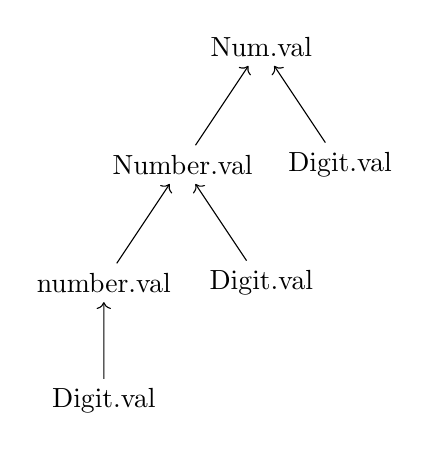
\begin{tikzpicture}
[level 1/.style={sibling distance=20mm},
 level 2/.style={sibling distance=20mm},<-,baseline]
  \node {Num.val}
  child {node {Number.val}
    child {node {number.val}
      child {node {Digit.val}}}
    child {node {Digit.val}}}
  child {node {Digit.val}};
\end{tikzpicture}  
\rmfamily
\item another example
\begin{grammar}
<decl> ::= <type> <var-list>

<type> ::= `int' \alt `float'

<var-list> ::= `id' `,' <var-list> \alt `id'
\end{grammar}

\begin{center}
\begin{tabular}{ll}
grammar Rule & semantic Rules\\
\hline
\(decl\to type\;var-list\) & \(var-list.dtype = type.dtype\)\\
\(type \to int\) & \(type.dtype = integer\)\\
\(type \to float\) & \(type.dtype = real\)\\
\(var-list1\to id,\;var-list2\) & \(id.dtype = var-list1.dtype\)\\
 & \(var-list2.dtype = var-list1.dtype\)\\
\(var-list \to id\) & \(id.dtype = var-list.dtype\)\\
\end{tabular}
\end{center}

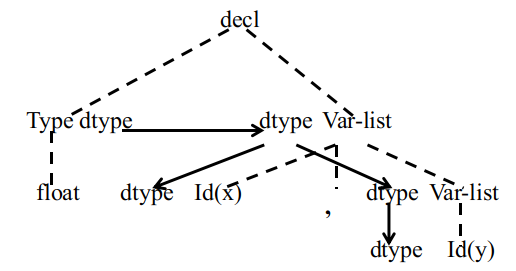
\includegraphics[width=100mm]{DeclDependencyGraph.png}
\item \textbf{directed acyclic graphs} DAG
topological sort
\end{itemize}

How attribute values are found at the roots of the graph
\begin{itemize}
\item \textbf{Parse tree method}: construction of the dependency graph is based on the
specific parse tree at compile time, add complexity and need circularity
detective
\item \textbf{Rule based method}: fix an order for attribute evaluation at compiler
construction time. It depends on an analysis of the attribute equations, or
semantic rules
\end{itemize}
\subsubsection{synthesized and inherited attributes}
\label{sec:orge76dd8b}
\begin{itemize}
\item \textbf{synthesized attributes}
\begin{itemize}
\item an attribute is synthesized if all its dependencies point from child to parent in
the parse tree
\item \textbf{S-attributed grammar}

an attribute grammar where all the attributes are synthesized
\end{itemize}
\item \textbf{inherited attributes}

inheritance from parent to siblings, from siblings to siblings.
\end{itemize}
\subsubsection{attributes as parameters and returned values}
\label{sec:orgf36f730}
\subsubsection{The use of external data structures to store attributes values}
\label{sec:org2f7af4d}
\begin{itemize}
\item Applicability
\begin{itemize}
\item Not suitable to the method of \textbf{parameters} and \textbf{returned values}
\item particularly when the attribute values have significant structure
and may be needed at arbitrary points during translation
\item Not reasonable to be stored in the syntax tree nodes
\end{itemize}
\item Ways:
\begin{itemize}
\item external data structures: table, graphs and other data structures. One
of the prime examples is the symbol table
\item replace attribute equations by calls to procedures representing
operations on the appropriate data structure used to maintain the
attribute values
\end{itemize}
\end{itemize}
\subsubsection{The computation of attributes during parsing}
\label{sec:org2c96381}
\begin{itemize}
\item \textbf{L-attributed}
\begin{itemize}
\item An attribute grammar of \(a_1,\dots,a_k\) is \textbf{L-attributed} if for each
inherited attribute \(a_j\) and each grammar rule \(X_0\to X_1\dots X_n\)
the associated equations for a\(_{\text{j}}\) are

\(X_i.a_j=f_{ij}(X_0.a_1,\dots,X_0.a_k,X_1.a_1,\dots,X_1.a_k,\dots,X_{i-1}
        .a_1,\dots,X_{i-1}.a_k)\)
\end{itemize}
\item \textbf{S-attributed grammar} is L-attributed
\item given an \emph{L-attributed} grammar where the \emph{inherited} attributes don't depend
on the \emph{synthesized} attributes
\begin{enumerate}
\item \textbf{Top-down parser}: a recursive-descent parser can evaluate all the
attributes by turning the inherited attributes into parameters and
synthesized attributes into returned values.
\item \textbf{Bottom-up parser}: LR parsers are suited to handling primarily
synthesized attributes, but are difficult for inherited attributes
\end{enumerate}
\item \(A\to B\;C\quad C.i=f(B.s)\) \emph{s} is a \emph{synthesized} attribute

\begin{center}
\begin{tabular}{ll}
Grammar Rule & Semantic Rules\\
\hline
\(A\to BDC\) & \\
\(B\to\dots\) & compute \(B.s\)\\
\(D\to\epsilon\) & \(saved_i=f(valstack[top])\)\\
\(C\to\dots\) & \(saved_i\) is available\\
\end{tabular}
\end{center}
\end{itemize}
\subsubsection{The dependence of attributes computation on the syntax}
\label{sec:org2ecdb77}
\textbf{Theorem}. Given an attribute grammar , \uline{all inherited attributes can be
changed into synthesized attributes} by suitable modification of the grammar,
without changing the language of the grammar. (Knuth[1968])


\subsection{The Symbol Table}
\label{sec:org8834d06}
\textbf{semantic checks} refer to properties of identifiers in the program - their
scope or type

\begin{center}
\begin{tabular}{llll}
NAME & KIND & TYPE & ATTRIBUTES\\
\hline
foo & fun & int * int -> bool & extern\\
\end{tabular}
\end{center}
\subsubsection{The structure of the symbol table}
\label{sec:orga39bbbf}
\begin{enumerate}
\item Linear list
\item Various search tree structures

AVL, B tree
\item hash tables

best choice

Collision resolution
\begin{enumerate}
\item open addressing
\item separate chaining
\end{enumerate}

The process of the hash function \(f:\Sigma^*\to\mathbb{N}/(size-1)\mathbb{N}\)

Good solution: repeatedly use a constant \(\alpha\) as multiplying factor

\(h_{i+1}=\alpha h_i+c_i, \quad h_0 = 0\)

Final hash value \(h=h_n\mod size\). Typically \(\alpha\) is a power of 2
\end{enumerate}
\subsubsection{Declarations}
\label{sec:org63af50a}
\begin{itemize}
\item constant declarations
\item type declarations
\item variable declarations
\item procedure/function declarations
\end{itemize}
\subsubsection{Scope rules and block structure}
\label{sec:org5b8835a}
two rules
\begin{itemize}
\item Declaration before use
\item the most closely nested rule for block structure
\end{itemize}
\subsubsection{interaction of same-level declarations}
\label{sec:orgabd07be}
\subsubsection{an extended example of an attribute grammar using a symbol table}
\label{sec:org9f891be}
\begin{grammar}
<S> ::= <exp> 

<exp> ::= `(' <exp> `)' \alt  <exp> `+' <exp>
\alt `id' \alt `num' \alt `let' <dec-list> `in' <exp>

<dec-list> ::= <dec-list> `,' <decl> \alt <decl>

<decl> ::= `id' `=' <exp>
\end{grammar}

Three attributes
\begin{itemize}
\item \texttt{err}: synthesize attribute. represent error
\item \texttt{symbol}: inherited attribute. represent the symbol table
\item \texttt{nestlevel}: inherited attribute, nonnegtive integer. represent the current
nesting level of the let blocks
\end{itemize}
\ttfamily
\begin{center}
\begin{tabular}{ll}
Grammar Rule & Semantic Rules\\
\hline
\emph{S \(\to\) exp} & exp.symtab = emptytable\\
 & exp.nestlevel = 0\\
 & S.err = exp.err\\
\hline
\emph{exp1 \(\to\) exp2+exp3} & exp2.symtab=exp1.symtab\\
 & exp3.symtab=exp1.symtab\\
 & exp2.nestlevel=exp1.nestlevel\\
 & exp3.nestlevel=exp1.nestlevel\\
 & exp1.err = exp2.err or exp3.err\\
\hline
\emph{exp1 \(\to\) (exp2)} & exp2.symtab =exp1.symtab\\
 & exp2.nestlevel =exp1.nestlevel\\
 & exp1.err = exp2.err\\
\hline
\emph{exp \(\to\) id} & exp.err = not isin(exp.symtab, id.name)\\
\hline
\emph{exp \(\to\) num} & exp.err = false\\
\hline
\emph{exp1 \(\to\) let dec-list in exp2} & dec-list.intab=exp1.symtab\\
 & dec-list.nestlevel=exp1.nestlevel+1\\
 & exp2.symtab=dec-list.outtab\\
 & exp2.nestlevel=dec-list.nestlevel\\
 & exp1.err = (dec-list.outtab=errtab) or exp2.err\\
\hline
\emph{dec-list1 \(\to\) dec-list2,decl} & dec-list2.intab= dec-list1.intab\\
 & dec-list2.nestlevel=dec-list1.nestlevel\\
 & decl.intab=dec-list2.outtab\\
 & decl.nestlevel=dec-list2.nestlevel\\
 & decl-list1.outtab=decl.outtab\\
\hline
\emph{dec-list \(\to\) decl} & decl.intab = dec-list.intab\\
 & decl.nestlevel=dec-list.nestlevel\\
 & dec-list.outtab=decl.outtab\\
\hline
\emph{decl \(\to\) id = exp} & exp.symtab = decl.intab\\
 & exp.nestlevel=decl.nestlevel\\
 & decl.outtab =\\
 & if(decl.intab = errtab)or exp.err\\
 & then errtab\\
 & else\\
 & if (lookup(decl.intab, id.name)= decl.nestlevel)\\
 & then errtab\\
 & else\\
 & insert(decl.intab,id.name,decl.nestlevel)\\
\end{tabular}
\end{center}
\rmfamily


\subsection{Data types and type checking}
\label{sec:orga57d00a}
\end{document}